\documentclass[a4paper]{report}
\usepackage[utf8]{inputenc}
\usepackage{amssymb}
\usepackage{amsmath}
\usepackage{amsthm} 
\usepackage{url}
\usepackage{xspace}
\usepackage{graphicx}
\usepackage[vlined]{algorithm2e} % lib for pseudo code
\usepackage{float}  % lib for pseudo code
\usepackage[T1]{fontenc}
\usepackage{pgfplots}
\usepackage{caption}
\usepackage{subcaption}
\usepackage{array}
\usepackage{mdframed}
\usepackage{rotating}
\usepackage{multirow}
\usepackage{dirtytalk}
\usepackage{longtable}
\usepackage[titletoc]{appendix}
\usepackage{hyperref}

\usepackage{listings}
\usepackage{color}

%New colors defined below
\definecolor{codegreen}{rgb}{0,0.6,0}
\definecolor{codegray}{rgb}{0.5,0.5,0.5}
\definecolor{codepurple}{rgb}{0.58,0,0.82}
\definecolor{backcolour}{rgb}{0.95,0.95,0.92}
\definecolor{lightgray}{rgb}{.9,.9,.9}
\definecolor{darkgray}{rgb}{.4,.4,.4}
\definecolor{purple}{rgb}{0.65, 0.12, 0.82}

\lstdefinelanguage{JavaScript}{
  keywords={typeof, new, true, false, catch, function, return, null, catch, switch, var, if, in, while, do, else, case, break},
  keywordstyle=\color{blue}\bfseries,
  ndkeywords={class, export, boolean, throw, implements, import, this},
  ndkeywordstyle=\color{darkgray}\bfseries,
  identifierstyle=\color{black},
  sensitive=false,
  comment=[l]{//},
  morecomment=[s]{/*}{*/},
  commentstyle=\color{purple}\ttfamily,
  stringstyle=\color{red}\ttfamily,
  morestring=[b]',
  morestring=[b]"
}

%Code listing style named "mystyle"
\lstdefinestyle{mystyle}{
  backgroundcolor=\color{backcolour},   commentstyle=\color{codegreen},
  keywordstyle=\color{magenta},
  numberstyle=\tiny\color{codegray},
  stringstyle=\color{codepurple},
  basicstyle=\footnotesize,
  breakatwhitespace=false,         
  breaklines=true,                 
  captionpos=b,                    
  keepspaces=true,                 
  numbers=left,                    
  numbersep=5pt,                  
  showspaces=false,                
  showstringspaces=false,
  showtabs=false,                  
  tabsize=2
}

%"mystyle" code listing set
\lstset{style=mystyle}


%Setup of the TableOfContent to incl. subsubsection
\setcounter{tocdepth}{3}
\setcounter{secnumdepth}{3}

\RestyleAlgo{boxruled}
\LinesNumbered


\newcolumntype{L}[1]{>{\raggedright\let\newline\\\arraybackslash\hspace{0pt}}m{#1}}

\graphicspath{ {Graphics/Images/} }

\usepackage{newunicodechar}
\newunicodechar{∙}{\cdotp}

\newcommand{\parahead}[1]{{\vspace*{6pt}\noindent\textbf{#1}\xspace\xspace\xspace\xspace}}

\newcommand{\heading}[1]{{\vspace{6pt}\noindent\sc{#1}}}

% Command for making <--> arrow with text above
\makeatletter
\newcommand\xleftrightarrow[2][]{%
  \ext@arrow 9999{\longleftrightarrowfill@}{#1}{#2}}
\newcommand\longleftrightarrowfill@{%
  \arrowfill@\leftarrow\relbar\rightarrow}
\makeatother

\newcommand{\dotp}[2]{\ensuremath{\left\langle {#1},{#2}\right\rangle}\xspace}
\newcommand{\Z}{\ensuremath{\mathbb{Z}}\xspace}
\newcommand{\Zq}{\ensuremath{\Z_q}\xspace}
\newcommand{\ZqStar}{\ensuremath{\Z_q^*}\xspace}
\newcommand{\Zp}{\ensuremath{\mathbb{Z}_p}\xspace}

\def\polyfactor{n\, \log_2^2 n}
\newcommand{\bigO}[1]{\ensuremath{\mathcal{O}\left(#1\right)}\xspace}
\renewcommand{\O}[1]{\ensuremath{{\mathcal{O}\left(#1\right)}}\xspace}


\theoremstyle{plain}
\newtheorem{thm}{Theorem}[subsection]
\newtheorem{lemma}{Lemma}[subsection]

\mdfdefinestyle{defstyle}{frametitlerule=true, frametitlerulewidth=0px}
\mdtheorem[style=defstyle]{defi}{Definition}[subsection]

\mdtheorem[style=defstyle]{infobox}{}[subsection]

\begin{document}

%***************************************************************
%               Title Page
%***************************************************************
\begin{titlepage}

\newcommand{\HRule}{\rule{\linewidth}{0.5mm}} % Defines a new command for the horizontal lines, change thickness here

\center % Center everything on the page
 
%----------------------------------------------------------------------------------------
%	HEADING SECTIONS
%----------------------------------------------------------------------------------------

\textsc{\LARGE Syddansk Universitet}\\[0.5cm] % Name of your university/college
\textsc{\large Data science}\\[1.5cm] %Minor Heading 


%----------------------------------------------------------------------------------------
%	TITLE SECTION
%----------------------------------------------------------------------------------------

\HRule \\[0.4cm]
{ \huge \bfseries Data science}\\[0.4cm] % Title
\HRule \\[1.5cm]
 
%----------------------------------------------------------------------------------------
%	AUTHOR SECTION
%----------------------------------------------------------------------------------------

\begin{minipage}{0.4\textwidth}
\begin{flushleft} \large
\emph{Author:}\\
Sune Chung \textsc{Jepsen} % Your name
Admir \textsc{Muric}\\ % Your name
Anna \textsc{\o}lgaard \textsc{Nielsen} % Your name
Veena \textsc{\o}lgaard \textsc{Nielsen} % Your name
Nevethan \textsc{\o}lgaard \textsc{Nielsen} % Your name
\end{flushleft}
\end{minipage}
~
\begin{minipage}{0.4\textwidth}
\begin{flushright} \large
\emph{Supervisor:} \\
Esmaeil S.  \textsc{Nadimi}\\ % Supervisor's Name
Jürgen   \textsc{Herp} \\% Supervisor's Name
Victoria   \textsc{Blanes‐Vidal} % Supervisor's Name
\end{flushright}
\end{minipage}\\[2cm]

% If you don't want a supervisor, uncomment the two lines below and remove the section above
%\Large \emph{Author:}\\
%John \textsc{Smith}\\[3cm] % Your name

%----------------------------------------------------------------------------------------
%	DATE SECTION
%----------------------------------------------------------------------------------------

{\large December 2017}\\[2cm] % Date, change the \today to a set date if you want to be precise

%----------------------------------------------------------------------------------------
%	LOGO SECTION
%----------------------------------------------------------------------------------------


\includegraphics{SDU_logo.png}\\[.5cm] % Include a department/university logo - this will require the graphicx package
 
%----------------------------------------------------------------------------------------

\vfill % Fill the rest of the page with whitespace

\end{titlepage}
%\chapter*{Acknowledgements}
%
It has been a learning period for the past six months, where we have studied the public verifiable secret sharing protocol. It has been a steep learning curve, but as we have worked with the topics on  a theoretical and practical level, we have gained an understanding of the protocol and its application.\\

\noindent
We would like to express our gratitude to our supervisor Ignacio Cascudo for his guidance and expert knowledge on this area throughout our work with this Master thesis. 

%\chapter*{Summary}
%In this Master thesis we will study the public verifiable secret sharing protocol and how it can be used in an electronic voting application based on the work from \cite{Schoenmakers1999}. Based on this knowledge we will design and implement a web based electronic voting application.\\

\noindent
Our work with this protocol leads to the following main topics which should cover our objective about Shamirs secret sharing, multiparty computation, public verifiable secret sharing protocol and our implementation of an electronic voting application.

\begin{enumerate}
    \item Voting
    \item Mathematical understanding
    \item Multiparty computation
    \item Electronic voting protocol
    \item Designing the application
    \item The application
    \item Reflection
\end{enumerate}

\noindent
We start with describing the concepts of electronic voting and the challenges with the different types of electronic voting applications. We will use other studies and their demands for concrete security requirements, which we can include in our consideration for our electronic voting application.  \\

\noindent
To understand the public verifiable secret sharing protocol one need some basic mathematical understanding and some knowledge about cryptographic tools. Modular arithmetic and group theory will be key elements in understanding how the protocol works. Regarding to the cryptographic tools we will present the discrete logarithm problem which is the security primitive for this protocol.\\

\noindent
Multiparty computation is basically about allowing parties to compute some function on some private inputs, in such a way that they learn the result but not the inputs from the other parties. Secret sharing is about hiding information in a random polynomial. By using this polynomial, parties can create shares based on evaluations in the polynomial. If enough parties then collect their shares together they will be able to recover the secret.  We will present a simple secret sharing example which illustrate how a secret can be distributed and reconstructed. In addition to these properties the public verifiable secret sharing protocol gives us the ability to publicly verify the validity of the shares among the parties involved in this protocol. This means that the protocol is secure against malicious parties which try to send votes which they are not supposed to do. \\

\noindent
The part describing the electronic voting protocol is divided into two parts, a basic and a more-in-depth description of the protocol. The first part is intended to supply enough basic knowledge for a software developer to implement a simple voting application based on the protocol. The second part is intended to give a more thorough insight of the protocol, here we describe the mathematical justifications behind the protocol as well as the proofs to verify the correctness and the consistency of the protocol. \\


\noindent
Designing the application is about architectural strategies for our application based on the knowledge from literature of \cite{Bass} and \cite{Baerbak10}. We took the security requirements of electronic voting in general as described in \cite{Cet09} as the functional demands for our application. To extract the architectural demands, such as \textit{Interoperability}, \textit{Modifiability} and \textit{Testability}, we used Quality attribute scenarios which is a way of defining a clear architectural measurable demands. In order to illustrate the impact these demands have on the architecture we will use several documentation methods here among diagrams. The process of deriving these demands is done through an Quality attribute workshop \cite{BarbacciQualityAttribute2003}. Since we have limited time we only used the structure of the Quality attribute workshop for deriving the Quality attributes scenarios without actually holding a workshop. Furthermore the structure of the workshop helped us prioritize among a long list of demands, and helped us derive the most important scenarios which we then proceeded on implementing.\\


\noindent
In the application part, we will elaborate on how we have implemented the final design of the architecture on a proof-of-concept application. \\

\noindent
Lastly the reflection part, summarizes the most important reflections on our results from the theoretical and the practical parts of this thesis. 



  


 

\clearpage

\tableofcontents


%***************************************************************
%               Part 1: Assignment
%***************************************************************
\chapter{Assignment} 
    \section{Assignment}

\subsection{Q-1: Boston Housing}

\subsubsection*{(a) Explore the Boston dataset in MASS library}
\begin{figure}[H]
\centering
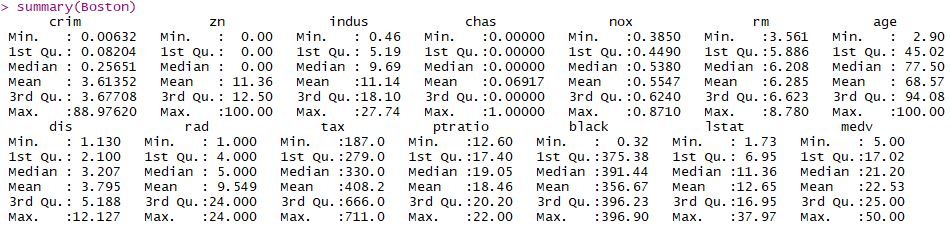
\includegraphics[scale=0.49]{Graphics/Assignment1/ExploreBoston.JPG}
\caption{Descriptive overview of Boston dataset}
\label{fig:logistic_regression_confusions_matrix_001}
\end{figure}


\subsubsection*{(b) Fit classification models}
\textbf{Logistic regression}





\iffalse
Step 1: Load data and run numerical and graphical summaries\\
Step 2: Split the data into training and testing data \\
Step 3: Fit a logistic regression model using training data\\
Step 4: Use the fitted model to do prediction for the test data\\
Step 5: Create the confusion matrix and compute the misclassification rate\\ \\
\fi


In figure \ref{fig:generalized_linear_model} the generalized linear model is explored. The features which are the most significant should be explored further. The algorithm outputs significant codes which results in the features with lowest p-values. The p-value expresses whether the null hypothesis should be accepted or rejected. If the the p value is less or equal to the significance level, there is strong evidence to reject the null hypothesis and accept the alternative hypothesis, $H_A$.   
In this case, the hypothesis expresses the influence of the predictor features to the predicted feature, which is the 'crim01'. The null hypothesis will be expressed as follows: $H_0 = 0$. 

The expression indicates that a specific predictor feature doesn't have a strong influence to the predicted feature. To find the features with importance to the predicted value, the null hypothesis has to be rejected, hence using the p value.    


\begin{figure}[H]
\centering
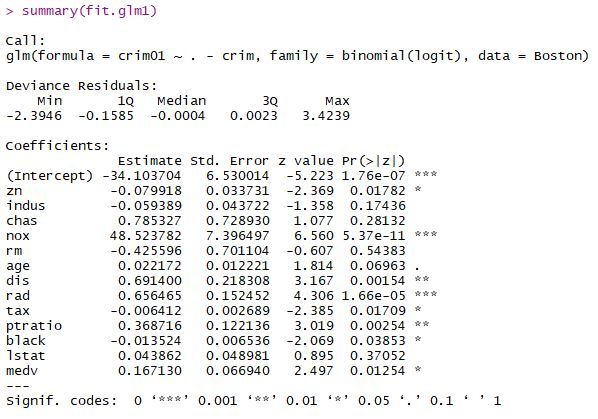
\includegraphics[scale=0.65]{LogisticRegressionCoefficientsExplore.JPG}
\caption{Generalized linear model}
\label{fig:generalized_linear_model}
\end{figure}

From the exploratory model, the following features which have a strong influence to the predicted value are: zn, nox, dis, rad, tax, ptratio, black and medv. 
All of these features are at a significance level of 0.05. In this experiment, other subsets of features will be used with different significance level. There are three subsets with different significance levels, 0.05, 0.01 and 0.001. The following features are at a significance level equal or less than 0.01: nox, dis, rad and ptratio. The last subset is for a significance level of 0.001: nox and rad.  

The misclassification of the models are computed with respect to the different subsets and their features with the training data as data input. Each model results in a confusion matrix. From the confusion matrix the misclassification rate and accuracy is computed by using formula from figure \ref{fig:confusion_Matrix} in the appendix.  \\

\begin{figure}[h]
\centering
\begin{minipage}{0.32\textwidth}
\centering
    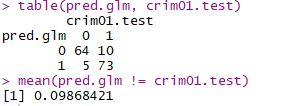
\includegraphics[width=\linewidth, height= 60pt]{LogisticRegressionConfusionsMatrix.JPG}
    \caption{Confusion Matrix - sign. level of 0.05}
    \label{fig:logistic_regression_confusions_matrix_005}
\end{minipage}\hfill
\begin{minipage}{0.32\textwidth}
\centering

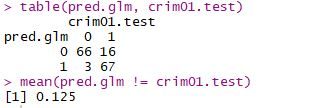
\includegraphics[width=\linewidth, height= 60pt]{LogisticRegressionConfusionsMatrix_001.JPG}
    \caption{Confusion Matrix - sign. level of 0.01}
    \label{fig:logistic_regression_confusions_matrix_001}
\end{minipage}\hfill
\begin{minipage}{0.32\textwidth}
\centering

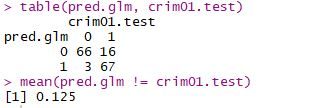
\includegraphics[width=\linewidth, height= 60pt]{LogisticRegressionConfusionsMatrix_001.JPG}
    \caption{Confusion Matrix - sign. level of 0.001}
    \label{fig:logistic_regression_confusions_matrix_001}
\end{minipage}
\end{figure}

The figures \ref{fig:logistic_regression_confusions_matrix_005}, \ref{fig:logistic_regression_confusions_matrix_001} and \ref{fig:logistic_regression_confusions_matrix_001} shows the different confusion matrices and error rates for each training of model in respect to their significance level\\

\\
\noindent
\textbf{LDA} \\
In the following experiment with Linear Discriminant Analysis (LDA), the same features with respect to the significance levels will be used for the model training. Just as before, each model has a confusion matrix and error rate.  

 



\begin{figure}[H]
\centering
\begin{minipage}{0.32\textwidth}
\centering
    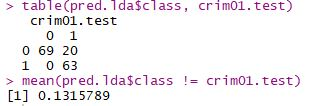
\includegraphics[width=\linewidth, height=50pt]{Graphics/Assignment1/LDAConfusionsMatrix_005.JPG}
    \caption{LDA Confusion Matrix - sign. level of 0.05}
    \label{fig:LDA_005}
\end{minipage}\hfill
\begin{minipage}{0.32\textwidth}
\centering

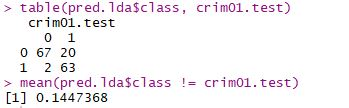
\includegraphics[width=\linewidth, height= 50pt]{Graphics/Assignment1/LDAConfusionsMatrix_001.JPG}
    \caption{LDA Confusion Matrix - sign. level of 0.01}
    \label{fig:LDA_001}
\end{minipage}\hfill
\begin{minipage}{0.32\textwidth}
\centering

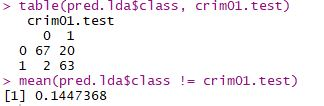
\includegraphics[width=\linewidth, height= 50pt]{Graphics/Assignment1/LDAConfusionsMatrix_0001.JPG}
    \caption{LDA Confusion Matrix - sign. level of 0.001}
    \label{fig:LDA_0001}
\end{minipage}
\end{figure}


\noindent
\textbf{KNN}\\
For this algorithm, the same subsets of features are used in relation to their significance level. Before the algorithm can be used with the subsets, the data set has to be normalized and the optimal \textit{k} values need to be found. In the process of finding the optimal k(s), a list of k's have been evaluated by using the \textit{class} package in R. It enables the use of the method \textit{knn()}. The optimal k(s) will be decided on their accuracy rates.

The process of normalizing data set and finding optimal k(s).\\
The data has been normalized into values between 0 and 1. Afterwards, the data has been used for training, where the accuracy of each \texttt{k} has been plotted. (Figure \ref{fig:optimal_ks})

\begin{figure}[H]
\centering
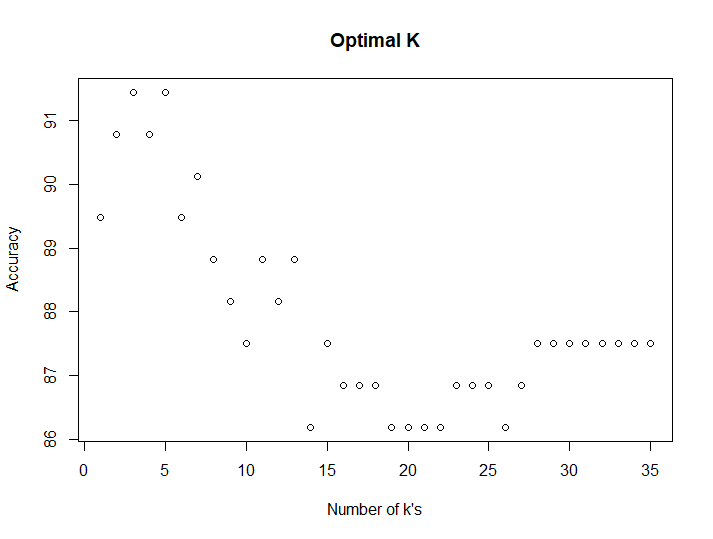
\includegraphics[scale=0.65]{Graphics/Assignment1/Rplot.png}
\caption{Plot of all k's}
\label{fig:optimal_ks}
\end{figure}

The process of training KNN with subsets \\
From the figure \ref{fig:optimal_ks}, the k values that have best accuracy 
 shows the code for the KNN training and how the subsets are used. The optimal k's in the experiment are 3 and 5. The training 




\subsubsection*{(c) Description of the findings}

\begin{table}[H]
\centering
\begin{tabular}{|c|c|c|c|}
\hline
Algorithm           & \begin{tabular}[c]{@{}c@{}}Significance \\ Level (\%)\end{tabular} & Accuracy (\%)                                                   & \begin{tabular}[c]{@{}c@{}}Misclassification \\ error rate (\%)\end{tabular} \\ \hline
Logistic Regression & 5                                                                  & 90.14                                                           & 9.86                                                                         \\ \hline
Logistic Regression & 1                                                                  & 87.5                                                            & 12.5                                                                         \\ \hline
Logistic Regression & 0.1                                                                & 88.2                                                            & 11.8                                                                         \\ \hline
LDA                 & 5                                                                  & 86.9                                                            & 13.1                                                                         \\ \hline
LDA                 & 1                                                                  & 85.2                                                            & 14.4                                                                         \\ \hline
LDA                 & 0.1                                                                & 85.5                                                            & 14.4                                                                         \\ \hline
KNN                 & 5                                                                  & \begin{tabular}[c]{@{}c@{}}(k=3) 93.2\\ (k=5) 92.8\end{tabular} & \begin{tabular}[c]{@{}c@{}}(k=3) 6.8\\ (k=5) 7.2\end{tabular}                \\ \hline
KNN                 & 1                                                                  & \begin{tabular}[c]{@{}c@{}}(k=3) 96.1\\ (k=5) 95.4\end{tabular} & \begin{tabular}[c]{@{}c@{}}(k=3) 3.9\\ (k=5) 4.6\end{tabular}                \\ \hline
KNN                 & 0.1                                                                & \begin{tabular}[c]{@{}c@{}}(k=3) 94.8\\ (k=5) 93.4\end{tabular} & \begin{tabular}[c]{@{}c@{}}(k=3) 5.2\\ (k=5) 6.6\end{tabular}                \\ \hline
\end{tabular}
\caption{Accuracy and Error rate in relation to significance level}
\label{table1}
\end{table}

It is important to note that LDA with CV = TRUE or FALSE, results the same.

\subsection{Q-2: Students Performance}

\subsubsection*{(a) Explicit model and probability for scoring an A}

To create an explicit model $L(\textbf{x})$ is calculated using the given $\beta_0$ and $\beta^T$ parameters. The \textbf{x} vector is a variable denoting the time invested in student's study and the student's grade point average. 

\begin{equation*}
    L(\textbf{x}) = \beta_0+\beta^T \textbf{x}=-6+[0.05,1]\begin{bmatrix}x_1 \\ x_2\end{bmatrix}
\end{equation*} 

The result of $L(\textbf{x})$ is put into the logistic regression model to be able to calculate probabilities of a student scoring an A at the exam. $\Pi_1$ will then represent the class of a student scoring an A and \textbf{x} a given student.

\textbf{Logistic Model:}
\begin{equation*}
\mathbb{P}(\Pi_1 | \textbf{x}) = \frac{e^{L(\textbf{x})}}{1+e^{L(\textbf{x})}} = \frac{e^{-6+[0.05,1][x_1, x_2]^T}}{1+e^{-6+[0.05,1][x_1,x_2]^T}}    
\end{equation*}

Given a student who studies 40 hours a week and has a grade point average of 3.5 (C+) the model is used to determine the probability of that student scoring an A at the exam by inserting the given information as $x_1$ and $x_2$.

\begin{equation}
\mathbb{P}(\Pi_1 | \textbf{x}) =  \frac{e^{-6+[0.05,1][40,3.5]^T}}{1+e^{-6+[0.05,1][40,3.5]^T}} =
\frac{e^{-0.5}}{1+e^{-0.5}} = 0.3775     
\end{equation}

The student has a 37.8 \% probability of getting an A at the exam.

\subsubsection*{(b) Weeks to study for 80\% chance of scoring an A}

Now the same student from the previous exercise wants to know how many hours of studying each week it will take to get a 80\% chance of getting an A to the exam.
To calculate the number of studying hours a week the probability of the logistic model is set to 0.8 and $L(\textbf{x})$ is isolated. Afterwards $x_1$, denoting weakly studying hours, will be isolated in the equation of $L(\textbf{x})$. 

\begin{align*}
\mathbb{P}(\Pi_1 | \textbf{x}) = \frac{e^{L(\textbf{x})}}{1+e^{L(\textbf{x})}} &= 0.8 \\
e^{L(\textbf{x})} &= 0.8*(1+e^{L(\textbf{x})}) \\
e^{L(\textbf{x})} &= 0.8 + 0.8*e^{L(\textbf{x})} \\
-0.8 &= 0.8*e^{L(\textbf{x})} - e^{L(\textbf{x})} \\ 
-0.8 &= -0.2*e^{L(\textbf{x})} \\
\frac{-0.8}{-0.2} &= e^{L(\textbf{x})} \\
ln(\frac{-0.8}{-0.2}) &= L(\textbf{x}) = 1.386 \\
& \\
L(\textbf{x}) = -6+[0.05,1]\begin{bmatrix}x_1 \\ 3.5\end{bmatrix}&=1.386 \\
-6+0.05*x_1+1*3.5&=1.386\\
0.05*x_1&=1.386+6-3.5\\
x_1=\frac{3.886}{0.05}&=77.72 hours \\
\end{align*}

A student with a grade point average of 3.5 (C+) needs to study 77.72 hours a week to have 80\% chance of scoring an A at the exam.


\section{Alcohol Related Car Crash}

\subsection{Identify demographic characteristics}
Identify the demographic characteristics of the drivers that are risk (or protective) factors of car accidents.

\subsection{Model}

Obtain the model relating BAC and car accidents (both, not adjusted and adjusted for confounders). 

Interpret the not‐adjusted and adjusted odds ratios. 

Is there a significant association between BAC and car accidents?

\subsection{Other potential confounder}
Is there any other potential confounder (not included in the file ”Data{_}car{_}accidents”) that should have
been considered in the study? 

How would you include it in the analysis?

\subsection{Unadjusted and adjusted models}

Plot the unadjusted (crude) and adjusted models. 
Comment on the similarities or differences between the
two.

\subsection{Probability}

What is the probability that a 40 yr male whose BAC is >1‰, causes a car accident? 

What will be the probability, 10, 20, 30 and 40 years later? Is this change linear?

\subsection{Predictive performance and the threshold value}

We obtain information on a new set of drivers (17 subjects). Evaluate the predictive performance of the model
by calculating the accuracy,sensitivity, specificity and precision of the model using this new data set.

Consider the threshold value for the probability as equal to 0.5. The data for the 17 subjects is in the Excel file ”

\section{Artist Identification}

%------------------ Start: Chapter intro -----------------
\subsection{Results}
\label{section:Results}
Following sub chapter shows the results, firstly the image is presented and it is followed by the results and a small explanation. Snippets of source code is in the appendix, however the full source code can be found in the \textcolor{blue}{\href{https://github.com/Spiderixius/DataScienceAssignments2017/tree/master/AssignmentEsmail}{Github repository}}, which will be made public Saturday the 16th of December 2017.
% Change the link to where ever the repo will be.

%------------------ End: Chapter intro -----------------


%------------------ Start: Image 1 -----------------
\subsubsection*{Image 1}

\begin{table}[H]
    \centering
    \caption{Predictions for Figure \ref{fig:renoir}.}
    \label{tbl:renoir_predictions}
    \begin{tabular}{lllll}
    \cline{1-4}
    \multicolumn{1}{|l|}{Renoir}         & \multicolumn{1}{l|}{Manet}          & \multicolumn{1}{l|}{Degas}          & \multicolumn{1}{l|}{Monet}          &  \\ \cline{1-4}
    \multicolumn{1}{|l|}{9.16161060e-01} & \multicolumn{1}{l|}{4.37439530e-06} & \multicolumn{1}{l|}{8.38107169e-02} & \multicolumn{1}{l|}{2.37891982e-05} &  \\ \cline{1-4}
                                         &                                     &                                     &                                     &  \\
                                         &                                     &                                     &                                     & 
    \end{tabular}
\end{table}


As seen in table \ref{tbl:renoir_predictions} we can see 9.16161060e-01 which is a 91.61\% certainty that it is a Renoir painting. Therefore the painting has been classified as drawn by Renoir.
%------------------ End: Image 1 -----------------



%------------------ Start: Image 2 -----------------
\subsubsection*{Image 2}

\begin{table}[H]
    \centering
    \caption{Predictions for Figure \ref{fig:outlier}.}
    \label{tbl:outlier_predictions}
    \begin{tabular}{lllll}
    \cline{1-4}
    \multicolumn{1}{|l|}{Renoir}         & \multicolumn{1}{l|}{Manet}          & \multicolumn{1}{l|}{Degas}          & \multicolumn{1}{l|}{Monet}          &  \\ \cline{1-4}
    \multicolumn{1}{|l|}{6.23026741e-10} & \multicolumn{1}{l|}{8.16067636e-01} & \multicolumn{1}{l|}{4.14584717e-03} & \multicolumn{1}{l|}{1.79786533e-01} &  \\ \cline{1-4}
                                         &                                     &                                     &                                     &  \\
                                         &                                     &                                     &                                     & 
    \end{tabular}
\end{table}

As seen by table \ref{tbl:outlier_predictions} we can see 8.16067636e-01 which is a 81.60\% certainty that it is a Manet painting. This is however not true as the painting was painted by Jackson Pollock, but such classification is not available in the output classifier, therefore it picks the next best thing, which seems to be Manet in this case. 
%------------------ End: Image 2 -----------------


%------------------ Start: Image 3 -----------------
\subsubsection*{Image 3}

\begin{table}[H]
    \centering
    \caption{Predictions for Figure \ref{fig:manet}.}
    \label{tbl:manet_predictions}
    \begin{tabular}{lllll}
    \cline{1-4}
    \multicolumn{1}{|l|}{Renoir}         & \multicolumn{1}{l|}{Manet}          & \multicolumn{1}{l|}{Degas}          & \multicolumn{1}{l|}{Monet}          &  \\ \cline{1-4}
    \multicolumn{1}{|l|}{2.28641890e-14} & \multicolumn{1}{l|}{1.00000000e+00} & \multicolumn{1}{l|}{1.85917379e-08} & \multicolumn{1}{l|}{4.80035141e-08} &  \\ \cline{1-4}
                                         &                                     &                                     &                                     &  \\
                                         &                                     &                                     &                                     & 
    \end{tabular}
\end{table}

As seen by table \ref{tbl:manet_predictions} we can see a whooping 1.00000000e+00 which is a 100\% certainty that it is a Manet painting. Therefore the painting has been classified as drawn by Manet.
%------------------ End: Image 3 -----------------



%------------------ Start: Image 4 -----------------
\subsubsection*{Image 4}

\begin{table}[H]
    \centering
    \caption{Predictions for Figure \ref{fig:degas}.}
    \label{tbl:degas_predictions}
    \begin{tabular}{lllll}
    \cline{1-4}
    \multicolumn{1}{|l|}{Renoir}         & \multicolumn{1}{l|}{Manet}          & \multicolumn{1}{l|}{Degas}          & \multicolumn{1}{l|}{Monet}          &  \\ \cline{1-4}
    \multicolumn{1}{|l|}{4.24926483e-10} & \multicolumn{1}{l|}{4.80975071e-03} & \multicolumn{1}{l|}{9.95190263e-01} & \multicolumn{1}{l|}{1.43515150e-13} &  \\ \cline{1-4}
                                         &                                     &                                     &                                     &  \\
                                         &                                     &                                     &                                     & 
    \end{tabular}
\end{table}


As seen in table \ref{tbl:degas_predictions} we can see a 9.95190263e-01 which is a 99.51\% certainty that it is a Degas painting. Therefore the painting has been classified as drawn by Degas.


%------------------ End: Image 4 -----------------



%------------------ Start: Solution Approach --------------
\subsection{Solution Approach}
The following section briefly describes the process that was committed to get the results for section \ref{section:Results}\\

\noindent{\textbf{Gather data:}} Data was gathered using a small Bash script [\ref{code:fetch_images}] to quickly download images for a certain artist. This process was repeated for all four artists.\\

\noindent{\textbf{Explore data:}} Gathered data was explored and it was apparent that Manet did not have more than 200 images. This information lead to the decision to use a maximum of 196 images for each artist, excluding the images from the assignment and a couple of images with errors in them. The reason to that was to prevent an artist from being too dominant. An example for a dominant factor would be using 1300 images which Renoir has within the style of impressionism. The 196 images for each artist was put into their own folders, with the artist name as the folder name.\\

\noindent{\textbf{Preparing the data:}} Gathered data was then prepared, for this Python was used. The code [\ref{code:load_data}] iterates through each four folders and process the images one by one. The dimension of the images is set to 224x224 which is a good balance between detailed and size to process. Afterwards the data was shuffled within each artist (not cross shuffle among artists) afterwards split into 80\% training data and 20\% test data [\ref{code:shuffle_and_split_data}]. The training and test data is then used for training and testing the convolutional neural network model.\\

\noindent{\textbf{Picking a pre-trained network:}} To avoid having to create a convolutional neural network from scratch it was decided to make use of an existing neural network. For this VGG16 [\cite{DBLP:journals/corr/SimonyanZ14a}] has been used that was pre-trained on ImageNet[\cite{imagenet_cvpr09}]. VGG16 consists of 16 convolutional neural networks.\\

\noindent{\textbf{Transfer Learning with VGG16:}} As mentioned in the previous paragraph an existing model is used, this is to avoid having to train the convolutional neural network from scratch and since there is only a maximum of 196 images per artist. Therefore transfer learning is made use of [\ref{code:model_creation_and_training}]. This happens in the following steps:
\begin{enumerate}
    \item Adjust image input to 224x224, the same dimension as our images from preprocessing
    \item Load VGG16 model pre-trained on ImageNet [\ref{fig:imagenet_vgg16}]
    \item Take VGG16's block5\_pool layers output.
    \item Feed the block5\_pool output to freshly created flatten layer.
    \item Create two fully connected layers with 128 neurons each, using RELU activation as the synapse.
    \item Create an output layer for four classes that makes use of softmax as the classifier
    \item Freeze all the layers except the newly added layers, this is to prevent the weights changing in the remaning layers
    \item Compile the new model which can then be used for training and test. [\ref{fig:custom_vgg16}]
    \item Train the model on the 80\% training data and then evaluate the model on the 20\% test data.
\end{enumerate}

The model is now ready to be used for classification of paintings that are not part of the test and training data. The model has an accuracy of 81.63\%. Not exactly the best to classify benign vs malignant tumor, however good enough for art :)



%------------------ End: Solution Approach --------------


    
%***************************************************************
%               Part 2: Alcohol related car crashes
%***************************************************************

\chapter{Alcohol related car crashes}
     

 
    

%***************************************************************
%               Part 3: Artist Identification
%***************************************************************
\chapter{Artist Identification}
    % Admir

% TODO:
% Collect all articles 
% Describe related apps (GoMore, CykelScore, ...)
% UX material design
% Other resources
%***************************************************************
%               Bibliography
%***************************************************************
\addcontentsline{toc}{chapter}{\\BIBLIOGRAPHY}
\bibliographystyle{alpha}
\bibliography{901_Bibliography}

\clearpage
%***************************************************************
%               Appendex
%***************************************************************
\appendix
\addcontentsline{toc}{chapter}{\\APPENDICES}
\chapter{Proofs}
\section{Assignment 1 images}

\label{app:confusion_matrix}
\begin{figure}[H]
\centering
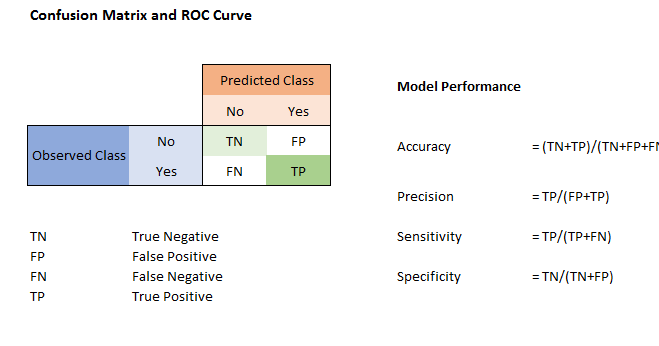
\includegraphics[scale=0.55]{Graphics/Assignment1/ConfusionMatrix.png}
\caption{Confusion Matrix}
\label{fig:confusion_Matrix}
\end{figure}

\subtitle{LDA coefficients results}
\begin{figure}[H]
\centering
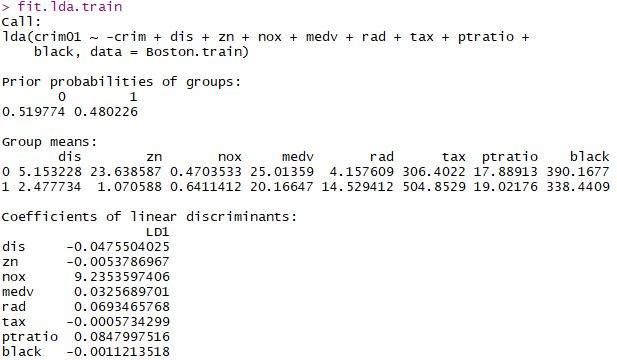
\includegraphics[scale=0.55]{Graphics/Assignment1/LDACoefficients_005.JPG}
\caption{Coefficients for significance level 5\%}
\label{fig:coefficients_method_005}
\end{figure}

\begin{figure}[H]
\centering
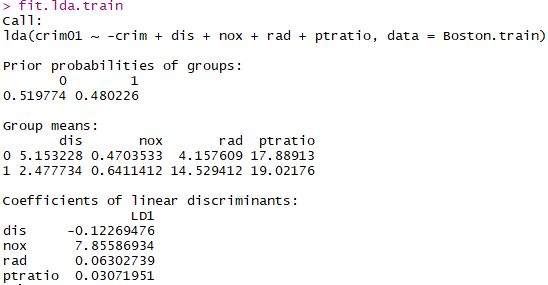
\includegraphics[scale=0.55]{Graphics/Assignment1/LDACoefficients_001.JPG}
\caption{Coefficients for significance level 1\%}
\label{fig:coefficients_method_001}
\end{figure}

\begin{figure}[H]
\centering
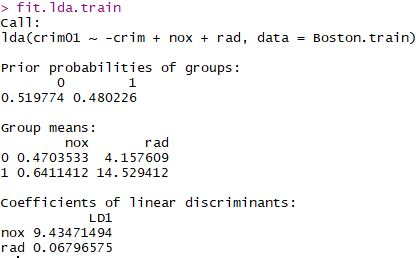
\includegraphics[scale=0.55]{Graphics/Assignment1/LDACoefficients_0001.JPG}
\caption{Coefficients for significance level 0.1\%}
\label{fig:coefficients_method_0001}
\end{figure}


\section{Assignment 3 images}
%--------------- Renoir Image -------------------------
\begin{figure}[H]
    \centering
    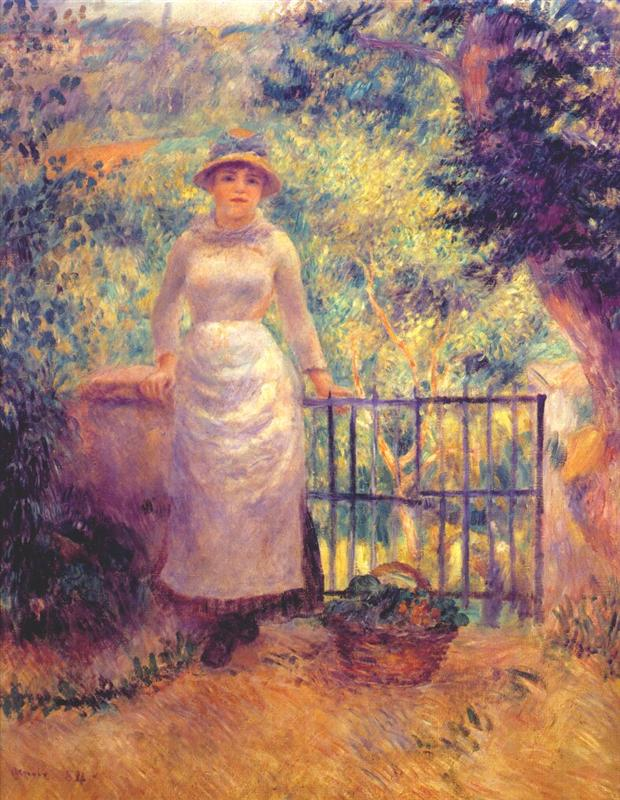
\includegraphics[scale=0.3]{Graphics/Assignment3/renoir.png}
    \caption{Pierre-Auguste Renoir: Aline at the gate.}
    \label{fig:renoir}
\end{figure}
%--------------- Outlier Image -------------------------

\begin{figure}[H]
    \centering
    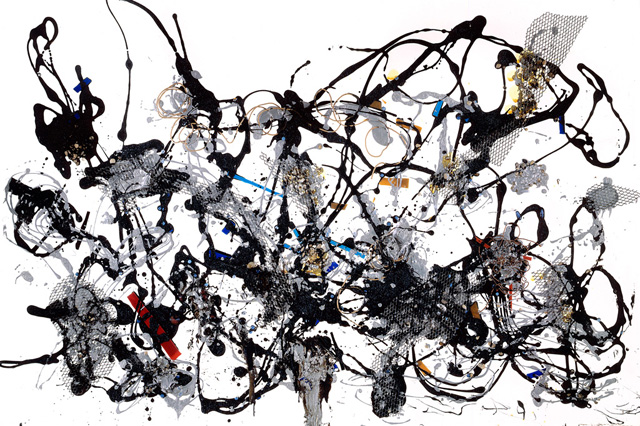
\includegraphics[scale=0.5]{Graphics/Assignment3/outlier.png}
    \caption{Jackson Pollock: Number 29.}
    \label{fig:outlier}
\end{figure}

%--------------- Manet Image -------------------------
\begin{figure}[H]
    \centering
    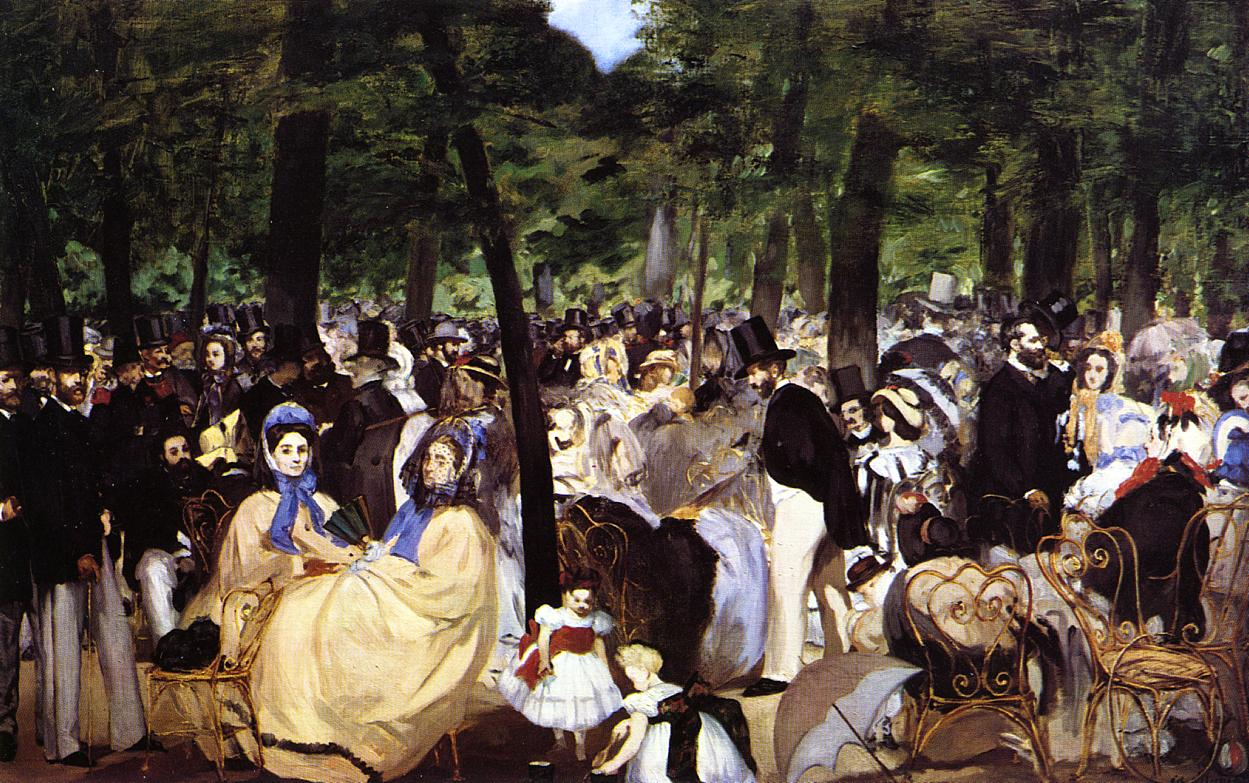
\includegraphics[scale=0.3]{Graphics/Assignment3/manet.png}
    \caption{Édouard Manet: Music in the Tuileries.}
    \label{fig:manet}
\end{figure}


%--------------- Degas Image -------------------------

\begin{figure}[H]
    \centering
    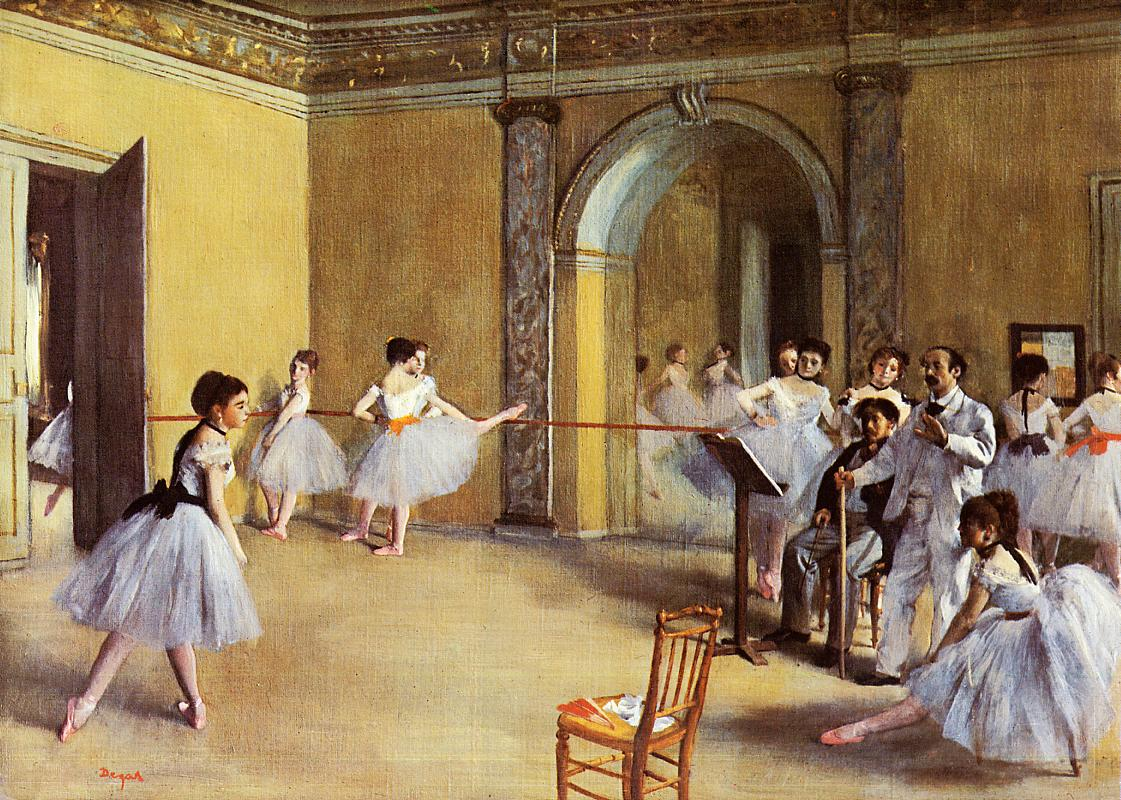
\includegraphics[scale=0.3]{Graphics/Assignment3/degas.png}
    \caption{Edgar Degas: Dance Class at the Opera.}
    \label{fig:degas}
\end{figure}

%--------------- VGG16 model Image -------------------------

\begin{figure}[H]
    \centering
    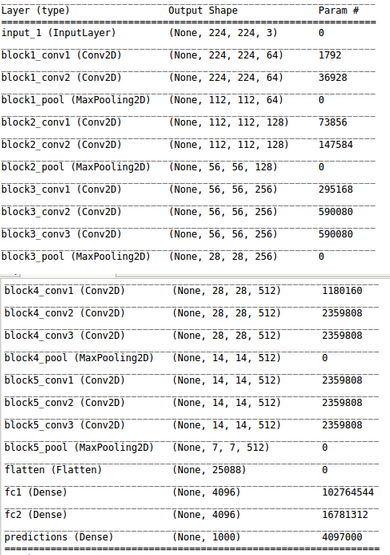
\includegraphics[scale=0.7]{Graphics/Assignment3/VGG16_model_image.png}
    \caption{VGG16 model with 1000 classes as output.}
    \label{fig:imagenet_vgg16}
\end{figure}

%--------------- Custom VGG16 model Image -------------------------

\begin{figure}[H]
    \centering
    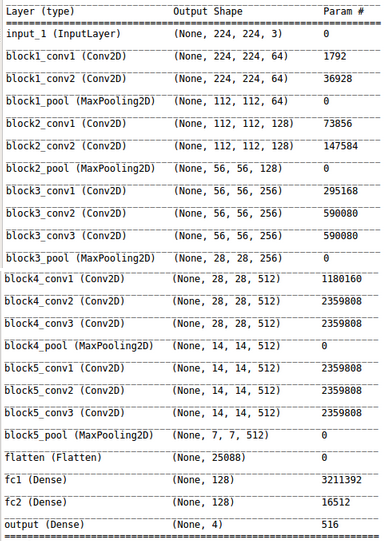
\includegraphics[scale=0.7]{Graphics/Assignment3/custom_model_image.png}
    \caption{Custom VGG16 model with 4 classes as output.}
    \label{fig:custom_vgg16}
\end{figure}

\section{Assignment 3 code}

%------------------ Fetch image code ----------------------
\begin{lstlisting}[frame=single, language=Bash, label={code:fetch_images}, caption={Code to fetch images from Wikiart for specific artists, in this case Manet.}]
    curl -s "https://www.wikiart.org/en/App/Painting/PaintingsByArtist?artistUrl=edouard-manet&json=2" | jq -r 'map(.image) | join("\n")' | sed '' | xargs -P 10 -n 1 curl -s -O
\end{lstlisting}

%------------------ Load data for preprocessing ---------------
\begin{lstlisting}[frame=single, language=Python, label={code:load_data}, caption={Code to load data for preprocessing.}]
    for dataset in data_dir_list:
	    img_list=os.listdir(data_path+'/'+ dataset)
    	for img in img_list:
    		img_path = data_path + '/'+ dataset + '/'+ img 
    		img = image.load_img(img_path, target_size=(224, 224))
    		x = image.img_to_array(img)
    		x = np.expand_dims(x, axis=0)
    		x = preprocess_input(x)
    		img_data_list.append(x)
\end{lstlisting}


%------------------- Shuffle and split into training and test --------------------
\begin{lstlisting}[frame=single, language=Python, label={code:shuffle_and_split_data}, caption={Code to shuffle and split the data to 80\% training and 20\% test.}]
#Shuffle the dataset
x,y = shuffle(img_data,Y, random_state=2)

# Split the dataset
X_train, X_test, y_train, y_test = train_test_split(x, y, test_size=0.2, random_state=2)
\end{lstlisting}

\begin{lstlisting}[frame=single, language=Python, label={code:model_creation_and_training}, caption={Code to load VGG16 pre-trained on ImageNet and doing transfer learning.}]
# Adjust the image input to 224, 224 and 3 channels
image_input = Input(shape=(224, 224, 3))

# VGG16 model
model = VGG16(input_tensor=image_input, include_top=True,weights='imagenet')

# Get VGG16's block5_pool layer and take its output
last_layer = model.get_layer('block5_pool').output
# Feed the output of block5_pool to the Flatten layer
x= Flatten(name='flatten')(last_layer)
# Create two fully connected layers with 128 neurons each, using RELU activation
x = Dense(128, activation='relu', name='fc1')(x)
x = Dense(128, activation='relu', name='fc2')(x)
# Create a output layer, using softmax classification
out = Dense(num_classes, activation='softmax', name='output')(x)
# Assign the new model to a variable
custom_vgg_model2 = Model(image_input, out)

# Freeze all the layers except the dense layers that was created above
for layer in custom_vgg_model2.layers[:-3]:
	layer.trainable = False

# Compile the new model architecture
custom_vgg_model2.compile(loss='categorical_crossentropy',optimizer='adadelta',metrics=['accuracy'])

# Time it
t=time.time()
# Train the model for 20 epochs using a batch size of 4
hist = custom_vgg_model2.fit(X_train, y_train, batch_size=4, epochs=20, verbose=1, validation_data=(X_test, y_test))
print('Training time: %s' % (t - time.time()))
# Test the model using accuracy as a metric
(loss, accuracy) = custom_vgg_model2.evaluate(X_test, y_test, batch_size=10, verbose=1)
print("[INFO] loss={:.4f}, accuracy: {:.4f}%".format(loss,accuracy * 100))
\end{lstlisting}





\end{document}
